\RequirePackage{fix-cm}
%
%\documentclass{svjour3}                     % onecolumn (standard format)
%\documentclass[smallcondensed]{svjour3}     % onecolumn (ditto)
%\documentclass[smallextended]{svjour3}       % onecolumn (second format)
\documentclass[twocolumn]{svjour3}          % twocolumn
\smartqed  % flush right qed marks, e.g. at end of proof
\usepackage{graphicx}

\usepackage{amssymb,amsmath}
%\newcommand{definition}{[Definition]}
%\newtheorem{definition}{Definition}
\DeclareMathOperator{\Ker}{Ker}
\DeclareMathOperator{\Supp}{Supp}

%\ifpdf \usepackage[pdftex]{graphicx} \pdfcompresslevel=9
%\else \usepackage[dvips]{graphicx} \fi

%\PrintedOrElectronic

% prepare for electronic version of your document
%\usepackage{t1enc,dfadobe}

%\usepackage{egweblnk}
\usepackage{cite}
\usepackage{algorithm}
\usepackage[noend]{algorithmic}
\usepackage{subfigure}
\usepackage{epsfig}
\usepackage{color}
\definecolor{turquoise}{cmyk}{0.65,0,0.1,0.1}
\definecolor{purple}{rgb}{0.65,0,0.65}
\newcommand{\tofix}[1]{{\color{green}[FIX: #1]}}
\newcommand{\ZQC}[1]{{\color{red}[Zhiquan: #1]}}
\newcommand{\YC}[1]{{\color{blue}[Yin: #1]}}
\newcommand{\YKL}[1]{{\color{magenta}[Yukun: #1]}}
\newcommand{\RRM}[1]{{\color{purple}[Ralph: #1]}}

% For backwards compatibility to old LaTeX type font selection.
% Uncomment if your document adheres to LaTeX2e recommendations.
\let\rm=\rmfamily    \let\sf=\sffamily    \let\tt=\ttfamily
\let\it=\itshape     \let\sl=\slshape     \let\sc=\scshape
\let\bf=\bfseries

\journalname{CGI2012} % The correct name will be entered by the editor
\begin{document}

\title{Generalized partial symmetry of shapes}
\subtitle{Insert your subtitle here, otherwise leave blank}
\author{First Author \and Second Author}
\institute{F. Author \at first adress \and S. Author \at second address}
\date{ }% The correct dates will be entered by the editor

\maketitle

\begin{abstract}
In this paper, we describe a new algorithm for detecting partial symmetry in shapes.
Our algorithm computes rigid symmetries, i.e., subsets of a shape that reoccur several times within the model differing only by translation, rotation or mirroring.
Our algorithm is based on matching locally coherent constellations of meaningful parts on the object surfaces.
In comparison to previous work, the new algorithm is able to detect partial symmetric parts without restrictions to regular patterns or nested hierarchies.
In addition, working on relevant meaningful parts only leads to a strong reduction in memory and processing costs such that very large data sets can be handled.
We apply the algorithm to a number of real world 2D and 3D scanner data sets, demonstrating high recognition rates for general partial symmetry.

\keywords{symmetry detection \and partial symmetry \and shape matching}
\end{abstract}

\section{Introduction}
\label{sec:introduction}

Building correspondences between two sets of features of 2D/3D shapes is a fundamental problem in many geometric processing,
computer graphics and computer vision tasks.
It arises in applications such as feature extraction~\cite{Johnson99,Lowe04,Sun09,Bokeloh08,Toler10,Leutenegger11},
shape matching~\cite{Berg05,Brown07,Lorenzo08,Tevs09,Ovsjanikov10,Tevs11,SahilliogluY11,Windheuser11}, registration of 3D shapes~\cite{Gelfand05,Aiger08,li08,Zeng10,vanKaick11,Chang11},
automatic shape understanding~\cite{Lipman09,Sun10,Kim11}, shape retrieval from database~\cite{Bronstein11}, and reconstruction~\cite{Brown07,Chang11}.

In principle and practise, the correspondence building process mainly proceed in three steps~\cite{Lowe04,Leutenegger11}:
salient feature detection, high-quality descriptor, and accurately matching.
The former two problems have been been widely attracted considerable attention as their importance is easy perceivable.
However, even with the ideal feature detector and descriptor that capturing the most important and distinctive information content enclosed in the detected salient regions,
the correspondences still could not ideally built in the state-of-the-art algorithms~\cite{vanKaick11}.
The reason is that the real input data is so inperfect and complex especially with symmetric and repetitive regions.
The researchers are beginning to be aware of that the limitation could be effectively alleviated by feature matching.
Some original idea (e.g. RANSAC-like algorithms~\cite{Tevs09,Tevs11}) has been extended,
or indirectly sorting to shape embedding strategies, such as Generalized Multidimensional Scaling~\cite{Bronstein11},
Heat Kernel Map~\cite{Ovsjanikov10}, M{\"o}bius Transformation~\cite{Lipman09,Kim11}.
But, these previous algorithms still did not treat feature matching as one independent problem,
although they agreed with that matching is not tightly coupled with feature detection and description.

In the paper, we mainly focus on feature matching problem, which is complementary to existing feature detection and desription algorithms.
As we know, a matching itself may comprise one or more items of a given kind.
We may match single point to single point (point-single),
point pairs separated by a fixed distance to other point pairs (segment-double),
triples of points forming a triangle to other triples of points (triangle-triple),
quadruples of points forming a quadrangle to other quadruples of points (quadrangle-quadruple), and so on.
As pointed by~\cite{Conte04}, when single features are matched,
we must solve a linear assignment problem, if multiple features are matched at once,
a quadratic or higher-order assignment problem results.

Linear assignment matches single features in one set with single features in the other set, and could be mainly treated as single points linkage.
Matching two feature sets by considering similarities of \emph{single} features from each set can easily fail in the presence of ambiguities such as repeated elements,
or similar local appearance.

Quadratic and higher-order assignment matches groups of features in one set simultaneously with groups from the other set,
and requires a greater consistency between the information being matched, making it more reliable.
As well as the features themselves, other constraints such as consistency of the distances between the features being matched are also enforced,
greatly improving the matching accuracy.

As a particular example of \emph{quadratic} assignment, Leordanu and Hebert~\cite{Leordeanu05} consider pairs of feature descriptors,
and distances between pairs of features from each set to reduce the number of incorrect correspondences.
Such pairwise distance constraints are particularly helpful in cases when the features themselves have low discriminative ability.
The idea has been widely adopted in the 3D shape matching algorithms~\cite{Tevs09,Ovsjanikov10,Tevs11,Kim11,SahilliogluY11,Windheuser11}.

Higher-order assignment further generalizes the assignment problem to include yet more complex constraints between features.
For example, third-order potential functions, proposed in~\cite{Duchenne09,Zeng10,Chertok10},
quantify the affinity between two point triples by measuring the similarity of the angles formed by such two feature tuples (triangles).
However, this angular similarity value only calculates the total differences in corresponding angles,
and does not change with the order of the input assignments.
By changing the affinity tensor to a \emph{supersymmetric} tensor~\cite{Kofidis02}, the unaccurate limitation could be further solved by our algorithm.

Thus, by formulating the higher-order problem using a supersymmetric affinity tensor,
we propose a general higher-order supersymmetric matching algorithm, named \emph{SuperMatching}.
SuperMatching, addressed in Section~\ref{sec:supersymhopm}, which accurately matching a moderate number of features using triples or higher polygons of features.
The contributions of this paper include:
\begin{itemize}
\item We show how to define a compact higher-order supersymmetric affinity tensor to express geometric consistency constraints between tuples of features.

\item Based on the supersymmetry of the affinity tensor, we propose a higher-order power iteration method, which efficiently solves the matching problem.

\item The affinity tensor is physically created by using a new efficient sampling strategy for feature tuples,
which avoids sampling repetitive items, reduces the number of feature tuples to be sampled while improving the matching accuracy.

\end{itemize}

Our experiments in Section~\ref{sec:experiments} on both synthetic and real captured data sets show that SuperMatching result is accurate and robust,
and has competitive computational cost compared to previous algorithms.
More important, the matching is performed by incorporating variant 2D and 3D feature descriptors,
which demonstrate that SuperMatching is independent on descriptors and could be generally applied in computer graphics and computer vision fields.

%Section~\ref{sec:supersymhopm} describes the higher-order supersymmetirc affinity tensor and the power iteration method.
%Experiments are shown in Section~\ref{sec:experiments} and conclusions drawn in Section~\ref{sec:conclusion}. 
\section{Related work}
\label{sec:related}

Finding correspondences between two sets of discrete features, such as points, is a classical problem, and thus there is a large literature on the subject.
Previous approaches can be classified into the which match single points to single points, those which match pairs of points to pairs of points, and so on.

Matching single points to single points, i.e.\ linear assignment problems, only consider affinity measures between two graph nodes, one from each set being matched, typically the feature distance between the two feature points.
In concrete terms, the linear assignment problem is posed as: find a mapping $f:\ P_1\to P_2$,
such that the optimal assignment $S^*=\argmax\sum\nolimits_{i\in P_1}A(i,j(i))$,
where $A:\ N_1\times N_2 \to R$ is the \emph{affinity matrix}, and $A(i,j)$ measures the affinity between feature $i\in P_1$ and feature $j\in P_2$.
%%%RRM Need to say the mapping is one to one?
Such affinity measures rely heavily on descriptors computed using local information around each feature point
(e.g.\ shape contexts~\cite{Belongie02}, SIFT~\cite{Lowe04}, spin images~\cite{Johnson99}, heat diffusion signatures~\cite{Sun09}) in many computer vision and geometric computing tasks.
It is apparent that point-to-point matching is weak in that wrong correspondences maybe readily be established.

Matching pairs of points in one set to pairs of points in the other set leads to a quadratic assignment problem.
We now have an affinity matrix $A: N_1N_2\times N_1N_2 \to R$, where $A(i,j)$ measures the compatibilities between two assignments $s_i=(f_i^1,f_{j(i)}^2)$ and $s_j=(f_i'^1,f_{j^{'}(i')}^2)$,
which takes into account both similarity of point features \emph{and} Euclidean distance between the points in a pair.
The quadratic assignment problem seeks to find a mapping $f:\ P_1\to P_2$ which represents the optimal assignment.
Unfortunately, this problem is NP-hard, but spectral relaxation techniques~\cite{Leordeanu05} can provide good approximate solutions.

Several higher-order constraints beyond pairwise potentials
%%%RRM why do you call them potentials? Not explained or defined yet.
have been proposed.
In general, we may define an $m^{th}$-order affinity measure $T_m$ to capture the affinity associated with making $m$ particular simultaneous assignments $s_{i_1}=(f_{i_1}^1,f_{j_1(i_1)}^2,),\; \cdots \;,s_{i_m}=(f_{i_m}^1,f_{j_m(i_m)}^2)$.
Such higher-order methods can significantly improve matching accuracy, 
but the higher-order assignment problem is again NP-hard, and various approximate methods have again been developed.
Zass and Sashua~\cite{Zass08} consider a probabilistic model of soft hypergraph matching.
They reduce the higher-order problem to a first-order one by marginalizing the higher-order tensor to a one dimensional probability vector.
Duchenne et al.~\cite{Duchenne_etal09} introduced a third-order tensor in place of an affinity matrix to represent affinities of feature triples,
and higher-order power iteration was used to achieve the final matching.
%%%RRM Need to say more here about how our method differs from this.
Chertok et al.~\cite{Chertok10} treat the tensor as a joint probability of assignments, marginalize the affinity tensor to a matrix,
and find optimal soft assignments by eigendecomposition of the matrix.
Wang et al.~\cite{Aiping10} also built a third-order affinity tensor and obtained a final matching by rank-one approximation of the tensor.
%%%RRM There are several methods above which we have used parts of. You need to
%%%RRM quite clearly say, for each paper seaparately
%%%RRM - which parts / ideas of these papers we have re-used
%%%RRM - how we have gone beyond them
Higher-order assignment problems typically require large amounts of memory and computational resources.
By reducing the number of elements needed to represent the affinity measures,
%%%RRM How is this reduction done?
the above approaches can efficiently match large numbers (many hundreds or more) of features.
However, these approaches sparsify the affinity information to some degree, leading to a reduction in matching accuracy.
When matching two feature sets with large differences in scale, the matching results may become unstable.
%%%RRM Why should the sets have large differences in scale? Surely most matching problems
%%%RRM are done with scale = 1?
%%%RRM Finish this by saying what our idea is that goes beyond these previous papers

A similar idea for 3D registration, called the 4-Points Congruent Sets method (4PCS), was proposed by Aiger et al.~\cite{Aiger08}. 
It is a fast and robust alignment scheme for 3D point sets that uses widely separated point tuples, providing resilience to noise and outliers.
The key geometric idea is that 4PCS defines a ratio property which is preserved for planar 4-point sets under affine transformations.
We use similar geometric rules in a more general way for feature matching.
%%%RRM be more specific about how we are more general.


\section{Algorithm}
\label{sec:alg}

Given one shape $\mathbb{S}$, our algorithm is mainly performed in three steps (illustrated by Figure~\ref{fig:Eager}): 1) automatically decompose the shape into some pieces, 2) for each piece $\mathbb{S}_i$, match the remaining shape $\mathbb{S}-\mathbb{S}_i$ to $\mathbb{S}_i$ such that for any node, a unique match from $\mathbb{S}_i$ is selected, 3) Put together all the correspondences to form a many-to-many correspondence in $\mathbb{S}$, and cluster nodes in $\mathbb{S}$ based on local consistency of the matching.

\begin{figure*}[t!]
\centering
  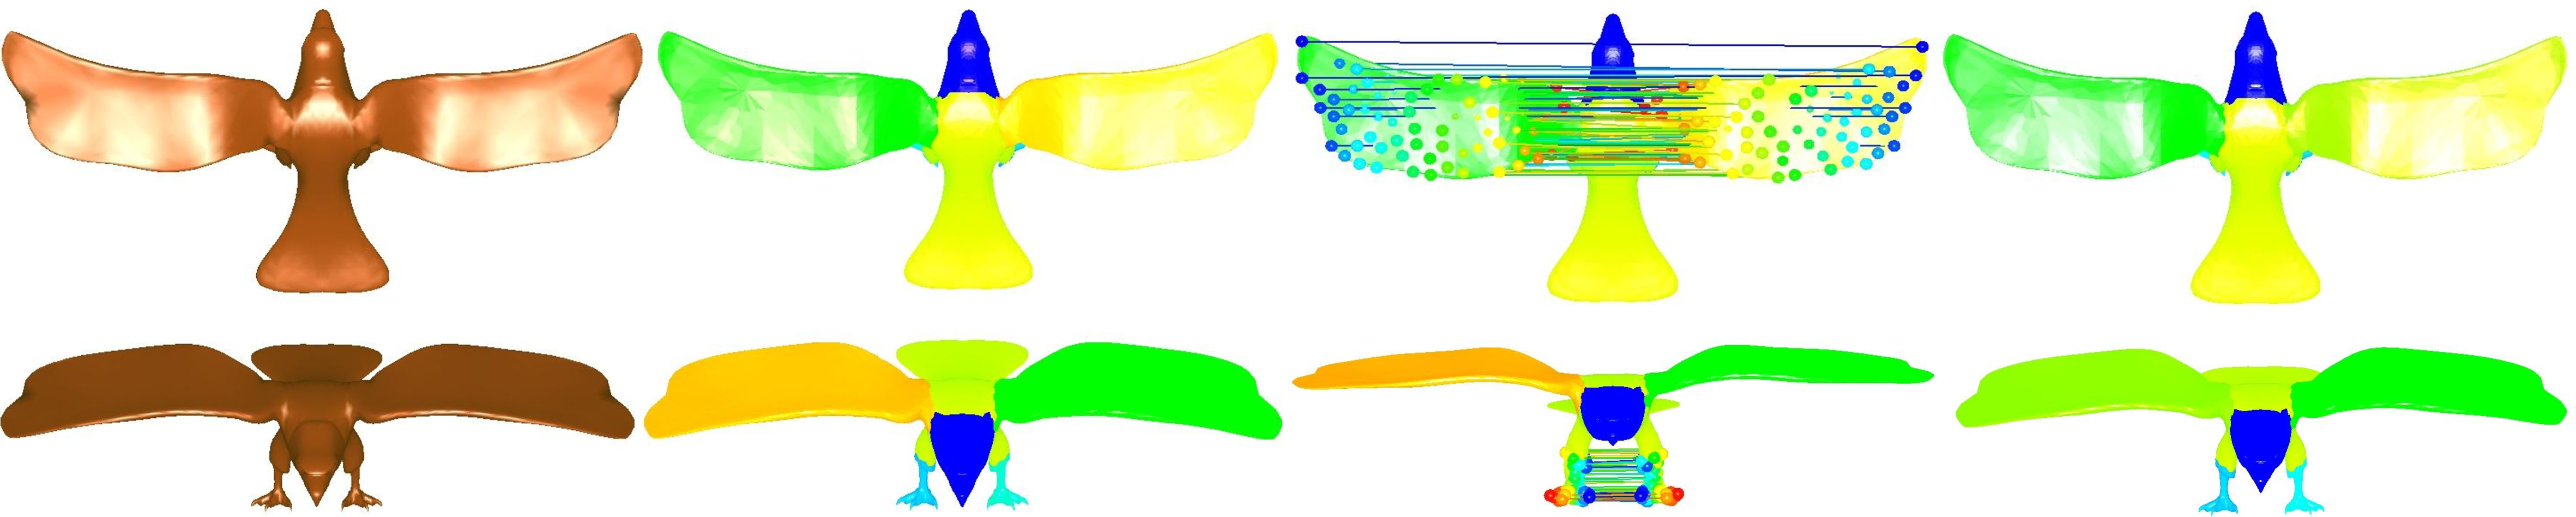
\includegraphics[width=0.99\linewidth]{figures/pipe.pdf}
  \caption{Algorithm pipeline.
  From left to right, for a given shape, our algorithm firstly decomposes it into several parts, matches each part to the remaining shape, then builds and clusters the correspondences based on the consistency of the matching. }
\label{fig:Eager}
\end{figure*}

\subsection{Automatic meaningful segmentation}
\label{subsec:segmentation}

For input shape $\mathbb{S}$, in order to find the generalized intrinsic partial symmetry, we decompose the model into $n$ pieces: $\mathbb{S}_1$, $\mathbb{S}_2$, $\dots$, $\mathbb{S}_n$.
The segmentation should ideally lead to each region representing a meaningful part of the object. We used random walks-based segmentation~\cite{lai2009} which involves distributing $n$ seeds as far away as possible over the surface and segmenting the shape based on hitting which seed with the maximum probability by a random walker starting from any face. The probability of movement is derived from the local geometry such that it is more difficult to move across sharp edges. Implied by the existing symmetry detection algorithms~\cite{xu2009,berner2011}, symmetric parts are always meaningful. This is the foundation of our algorithm and could explain why the meaningful segmentation is first performed to provide the parts for symmetry detection.

\subsection{Partial matching}
\label{subsec:matching}

In order to find the symmetries, we uniformly sample the shape $\mathbb{S}$ with $m$ samples, 
and then build the partial matching between every pair of regions $\mathbb{S}_i$ and $\mathbb{S}_j$, $i \neq j$. 

The partial matching is achieved by a third-order tensor matching algorithm [reference omitted for review],
which is improved from the tensor-based algorithm for high-order graph matching~\cite{Duchenne2011}.
Our algorithm formulates the matching using a supersymmetric tensor representing an affinity metric,
which takes into account feature similarity and geometric constraints between features.
Note that, although~\cite{Duchenne2011} claimed to use a supersymmetric affinity tensor, 
their approach did not make full use of supersymmetry when creating the supersymmetric affinity tensor, nor does it take advantage of supersymmetry
to accelerate the power iteration process and sampling.
Going beyond~\cite{Duchenne2011}, our algorithm [reference omitted for review] really takes advantage of supersymmetry to devise an
efficient sampling strategy to estimate the affinity tensor, as well as to store the estimated tensor compactly.
Matching is performed by an efficient higher-order power iteration approach which takes advantage of the compact representation of the supersymmetric affinity tensor.
efficient sampling strategy to estimate the affinity tensor, as well as to store the estimated tensor compactly.
Matching is performed by an efficient higher-order power iteration approach which takes advantage of this compact representation.

The algorithm matches samples using a pair of three-tuples from both shapes and ensures consistency in geodesic distances. 
Assume the number of matches between regions $\mathbb{S}_i$ and $\mathbb{S}_j$ is $match_{i,j}$, 
the regions are recognized as of candidate symmetry if $match_{i,j} > cm$, where $c$ is a constant and typically assigned as $0.2/n$ for all tested examples in the paper.

\subsection{Correspondences clustering}

In the following, we put together all the correspondences for each part $\mathbb{S}_i$, found by former partial matching.
So, we form a many-to-many correspondence in the whole $\mathbb{S}$.  
Then, we cluster nodes in $\mathbb{S}$ based on local consistency of the matching.
Benefiting from our partial matching, rigid transforms can be computed from each triple of compatible matching points.
The transform which brings the most data points within a threshold distance of a point in the model is chosen as the optimal alignment transform~\cite{Huttenlocher1990}.
As shown by ~\cite{Huttenlocher1990}, this transformation always exists for three non-collinear points, and is unique up to a reflective ambiguity. 
The solution method is closed-form and only involves second-order equations.
The later paper~\cite{Gelfand05} claimed that such a voting scheme is robust to the initial pose of the triples.
Our clustering method is similar to~\cite{mitra2006} based on the computed transformation that map local surface patches onto each other.
Each matching pair provides evidence for a symmetry relation at the level of the local sample spacing. 
So, we could extract meaningful symmetries at larger scales by finding groups of pairs with a similar transformation 
that correspond to symmetric subsets of the shape.




\section{Results}
\label{sec:result}

Our algorithm is tested on a variety of 3D shapes. 
We visualize the discrete matches using the similar color as the corresponding symmetry parts.

We first show experimental results on clean manifold meshes, which are not corrupted with noise, and are complete. 
For such models, our algorithm provides good segmentation for the partial matching, and we reliably obtain perfect results (e.g. Figure~\ref{fig:Eager} and~\ref{fig:Tiger}). 

\begin{figure}[t]
\centering
  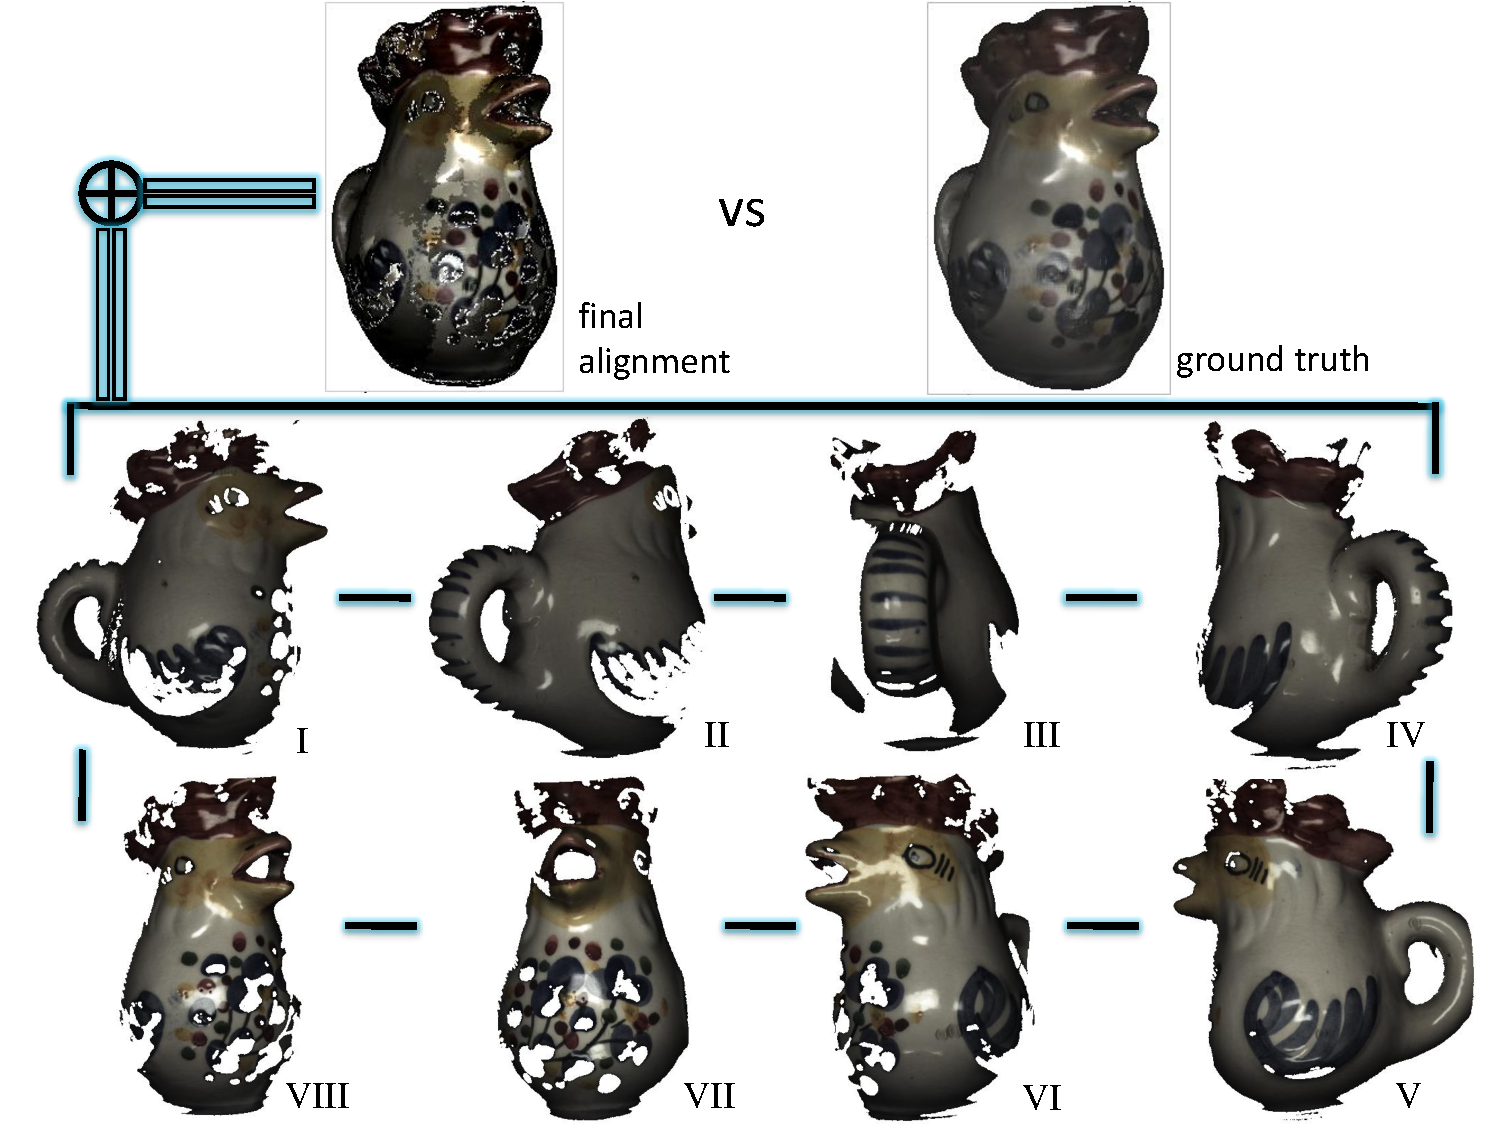
\includegraphics[width=0.99\linewidth]{figures/Rooster.pdf}
  \caption{The four legs could be detected as one symmetric region at the current configuration $c=0.2/n$.
  It is mainly resulting from the large similarity of four legs.}
\label{fig:Tiger}
\end{figure}

As our algorithm works on the meaningful segmentation, uniform sampling, and clustering, the matching results do not depend on the tessellation of the shapes.
Figure~\ref{fig:Point} demonstrates that our algorithm performs very well on the shape in the point set form.

\begin{figure}[t]
\centering
  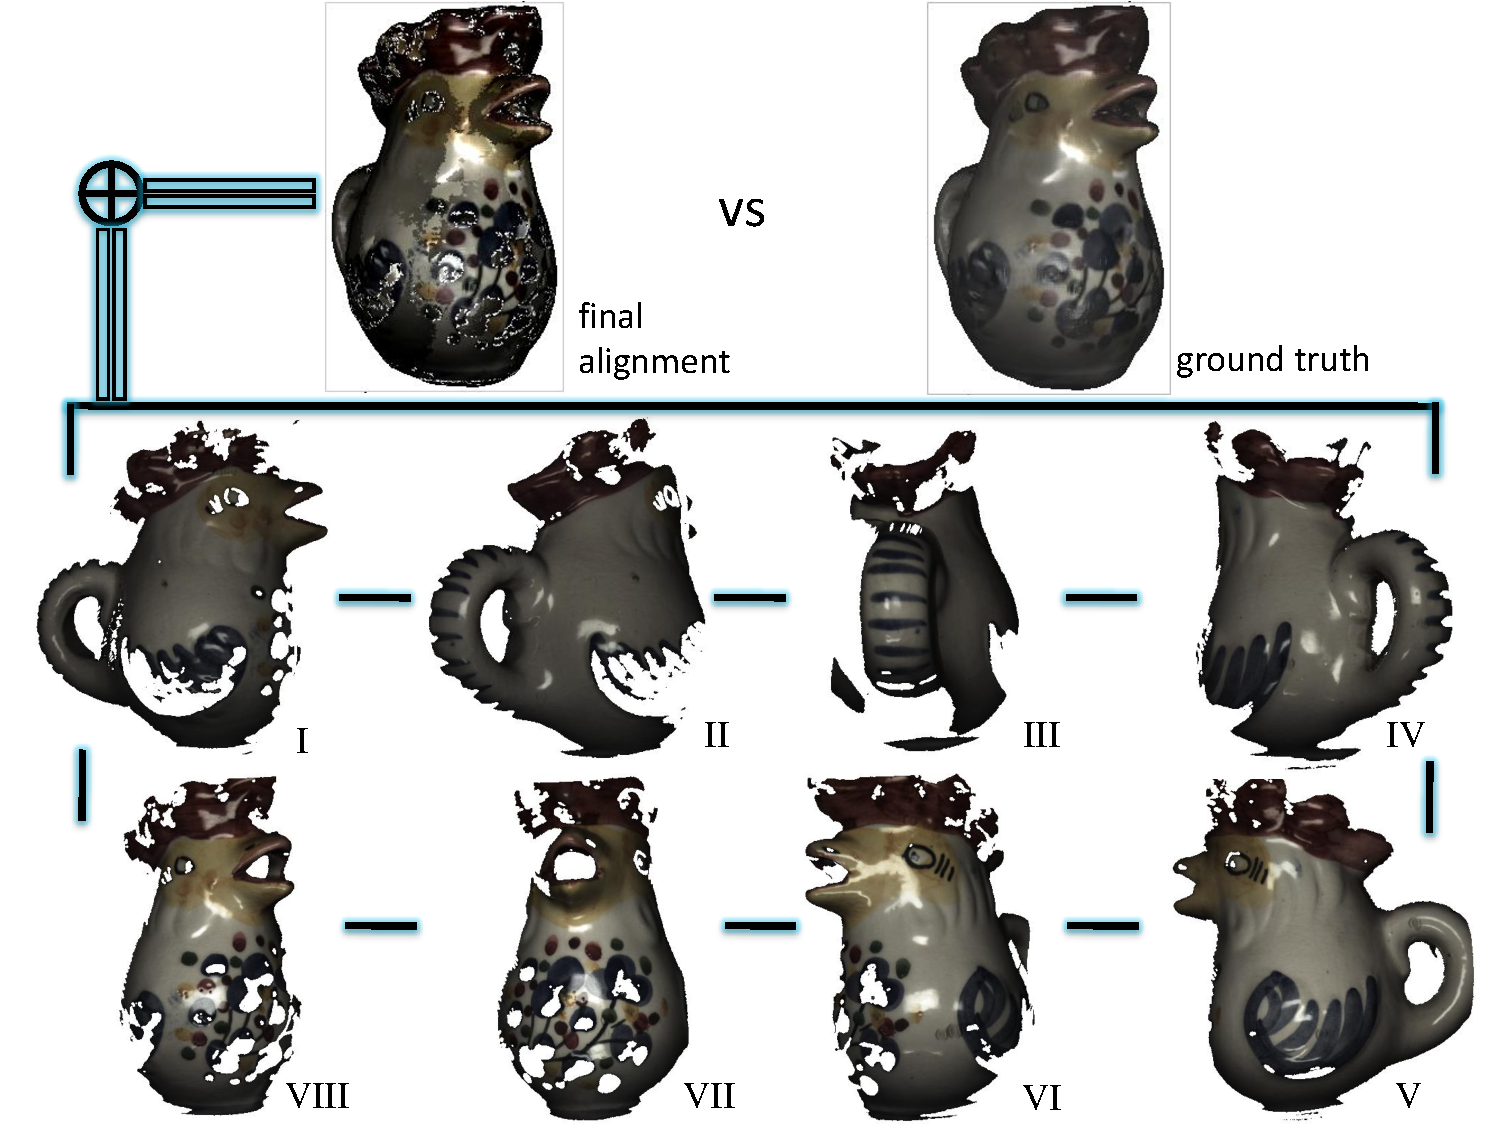
\includegraphics[width=0.99\linewidth]{figures/Rooster.pdf}
  \caption{The in point set form.}
\label{fig:Point}
\end{figure}

Figure~\ref{fig:Gargoyl} shows an example using the three different symmetry group composed of reflection, rotation, and translation.
The symmetry is detected in coarse-to-fine steps based on the hierarchical segmentation.
In the coarse level, all major reflection symmetries are faithfully recovered.
While in the fine level, most rotation and translation symmetries are detected.
Note that, the example is clearly claimed as the failure case in the STAR algorithm~\cite{berner2011}.

We use another example on the complete and non-complete Armidillo (Figure~\ref{fig:Arm}) to demonstrate the robustness of our algorithm.
Both on the complete and non-complete cases, the algorithm computes a global reflectional plane based on all final correspondences. 
Experiments show that the plane is almost same in the both cases.

\begin{figure}[t]
\centering
  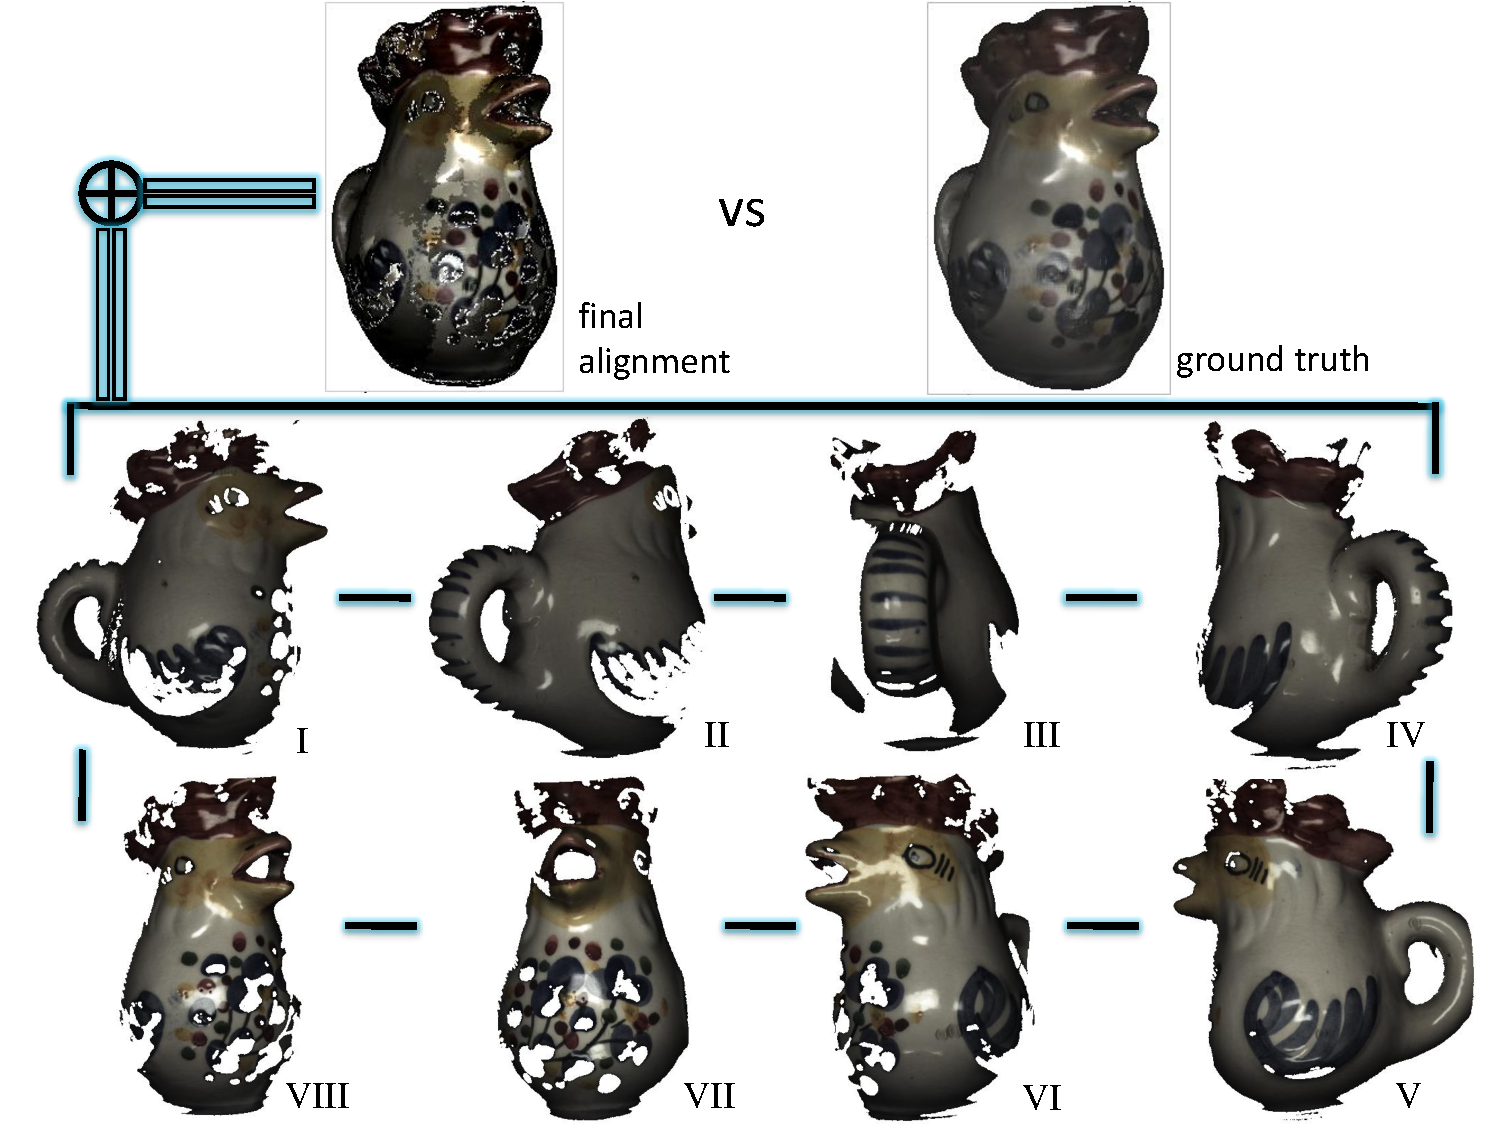
\includegraphics[width=0.99\linewidth]{figures/Rooster.pdf}
  \caption{The global reflectional planes are computed from the complete and non-complete Armadillo shapes.}
\label{fig:Arm}
\end{figure}

The performance data of Table 1 indicates how the computation on the symmetries of the shapes.

\begin{table*}
\centering
\begin{tabular}{l|r|r|r|r|r}
Model
& Vertices
& Parts number
& Segmentation
& Partial matching
& Correspondences clustering \\
\hline
%%%RRM Use captial letter for all model names
Armadillo  & 172,974  & 9 &  982ms   & 2ms & 7ms \\
bumpy plane&   3,721  & 14 & 47ms     & 1ms & 2ms  \\
Eager      &  14,618  & 6 & 413ms    & 2ms & 3ms \\
Gargoyl    & 250,003  & 6 & 218ms    & 3ms & 3ms  \\
%feline     &  49,864  & 20 & 109ms    & 3ms & 2ms \\

\hline
\end{tabular}
\caption{Timing for our algorithm: automatic meaningful segmentation, partial matching of each part,
and clustering the correspondences, using a 1.6GHz Intel Core i7CPU laptop with 4GB of RAM.
}
\label{tab:timing}
\end{table*}
\section{Conclusions}
\label{sec:con}

We have proposed a symmetry detection algorithm for discovering and extracting partial symmetries of 3D geometric models.
The algorithm could detects the general symmetry types, such as the rotation, translation, and mirroring symmetry.
It is robust as relying on the shape segmentation, and shows the advantage over the graph matching using salient feature lines.
Our algorithm is provably effective, easy to implement, and applicable to a wide range of 3D shapes.

\paragraph{Discussion.} 
The main limitation of our symmetry detection algorithm stems from the foundation that we build it by using the segmentation algorithm.
In presence of significant noise, this assumption breaks down for our choice of meaningful segmentation, 
thus forcing the algorithm to the unstable scenario.
As the rapid development and maturity of meaningful segmentation~\cite{Shamir2008}, 
more segmentation algorithm would and could be employed to produce more reasonable decomposition.
In addition, it is useful and necessary to develop more efficient algorithm by resorting to multi-resolution or parallelization
techniques (e.g., using the GPU) to improve the speed of the algorithm.


\bibliographystyle{ieeetr}
\bibliography{parsym}
\end{document}


